\documentclass[12pt]{article}

\usepackage{sbc-template}
\usepackage{graphicx,url}
\usepackage[utf8]{inputenc}
\usepackage[brazil]{babel}
  

     
\sloppy

\title{ESP32-LLM Benchmark: Uma Avaliação Experimental da Confiabilidade de Código para Sistemas Embarcados Gerado por Large Language Models}

\author{Renato William Rodrigues de Souza\inst{1}}

\address{Instituto Federal de Educação, Ciência e Tecnologia do Ceará (IFCE)\\
Campus Boa Viagem -- Boa Viagem -- CE -- Brasil
}

\begin{document} 

\maketitle

\begin{abstract}
This study evaluates the reliability of ESP32 code generated by three Large Language Models (LLMs) across different levels of task difficulty. A benchmark composed of 30 tasks derived from a real embedded-system firmware was defined, with 10 easy, 10 medium, and 10 hard tasks. The same standardized prompts were submitted to GPT-5.6-Sol, DeepSeek-V4-Pro, and Claude-Sonnet-5, resulting in 90 generated solutions. The evaluation combined compilation, automated functional tests, qualitative assessment, and statistical analysis. The results indicate high performance on easy and medium tasks, while a marked degradation was observed on hard tasks. No statistically significant differences were found among the models regarding compilation or overall functional performance, whereas task difficulty had a significant effect for all three LLMs. The findings also show that highly rated qualitative solutions may still fail to compile or integrate correctly in the target firmware.
\end{abstract}
     
\begin{resumo}
Este trabalho avalia a qualidade de código ESP32 gerado por três Large Language Models (LLMs) em diferentes níveis de dificuldade. Foi definido um benchmark composto por 30 tarefas derivadas de um firmware real de sistema embarcado, sendo 10 fáceis, 10 médias e 10 difíceis. Os mesmos prompts padronizados foram submetidos ao GPT-5.6-Sol, DeepSeek-V4-Pro e Claude-Sonnet-5, totalizando 90 soluções geradas. A avaliação combinou compilação, testes funcionais automatizados, análise qualitativa e análise estatística. Os resultados indicaram elevado desempenho nas tarefas fáceis e médias, mas forte queda nas tarefas difíceis. Não foram observadas diferenças estatisticamente significativas entre os modelos quanto à compilação ou ao desempenho funcional global, enquanto o nível de dificuldade apresentou efeito significativo para as três LLMs. Os resultados também mostram que soluções qualitativamente bem avaliadas podem ainda falhar na compilação ou na integração com o firmware alvo.
\end{resumo}


\section{Introdução}
\label{sec:introducao}

Os avanços recentes em Large Language Models (LLMs) ampliaram o uso desses modelos em atividades de Engenharia de Software, incluindo geração, completação e transformação de código. A capacidade de produzir implementações a partir de descrições em linguagem natural motivou a criação de benchmarks destinados a mensurar a correção funcional do código gerado. Entre os trabalhos de referência, HumanEval e MBPP consolidaram a avaliação baseada na execução de casos de teste como uma das principais formas de investigar essa capacidade \cite{chen2021codex,austin2021program}. Estudos posteriores mostram que a avaliação de LLMs para geração de código permanece fortemente associada a benchmarks e métricas de correção funcional \cite{umama2025slr}.

Embora esses benchmarks sejam fundamentais para a comparação entre modelos, tarefas algorítmicas relativamente autocontidas não representam integralmente as condições encontradas no desenvolvimento de software embarcado. Nesse domínio, uma solução pode depender de bibliotecas específicas, APIs de hardware, estruturas de dados, variáveis globais, estados compartilhados e contratos de integração com outras partes do firmware. Estudos sobre o uso de LLMs no desenvolvimento e depuração de sistemas embarcados evidenciam que a interação entre software, hardware e ambiente de execução introduz desafios que não são adequadamente representados por tarefas puramente algorítmicas \cite{englhardt2023embedded}. Consequentemente, código aparentemente correto quando analisado isoladamente pode apresentar problemas quando submetido à compilação, execução ou integração no sistema alvo. Essa característica reforça a importância de avaliações que considerem evidências executáveis e múltiplas dimensões da qualidade do código gerado \cite{nogueira2026probe}.

Investigações recentes começaram a explorar essa questão no contexto de sistemas embarcados. Babiuch e Smutny avaliaram diferentes LLMs em cenários de programação de sistemas baseados em microcontroladores e aplicações IoT, incluindo o ESP32, evidenciando a importância da complexidade das tarefas nesse tipo de avaliação \cite{babiuch2026benchmarking}. Paralelamente, trabalhos sobre qualidade de código e avaliação multidimensional indicam que a análise de soluções geradas por LLMs não deve se restringir a uma única perspectiva \cite{patcas2026quality,nogueira2026probe}. Nesse cenário, permanece relevante investigar o comportamento desses modelos quando as tarefas são derivadas de componentes reais de firmware e possuem diferentes graus de dependência do contexto do sistema.

Este trabalho apresenta o \textit{ESP32-LLM Benchmark}, um estudo experimental para avaliar a confiabilidade de código ESP32 gerado por LLMs. Neste estudo, confiabilidade é operacionalizada como a capacidade de a solução gerada compilar, satisfazer testes funcionais previamente definidos e preservar os contratos necessários para integração com o firmware alvo. O benchmark foi construído a partir de um firmware real de uma estação de monitoramento baseada em ESP32 e compreende 30 tarefas distribuídas igualmente entre três níveis de dificuldade. Três LLMs foram submetidas aos mesmos prompts, sem ciclos de correção ou refinamento, produzindo um conjunto de 90 soluções para avaliação.

O estudo é orientado por quatro questões de pesquisa: \textbf{RQ1}: Como as LLMs avaliadas diferem quanto à capacidade de gerar código ESP32 compilável e funcionalmente correto? \textbf{RQ2}: Em que medida o nível de dificuldade das tarefas afeta a correção funcional do código ESP32 gerado pelas LLMs? \textbf{RQ3}: Em que medida avaliações qualitativas do código gerado estão associadas ao seu desempenho objetivo de compilação e testes funcionais? \textbf{RQ4}: Quais são os principais tipos de falha encontrados nas soluções geradas para tarefas de maior dificuldade?

As principais contribuições deste trabalho são: (i) a definição de um benchmark com 30 tarefas extraídas de um firmware ESP32 real e organizadas em três níveis de dificuldade; (ii) a avaliação experimental de 90 soluções produzidas por três LLMs sob um protocolo padronizado; (iii) a combinação de compilação, 151 casos de teste funcionais e avaliação qualitativa cruzada; e (iv) a análise do efeito da dificuldade, da relação entre avaliação qualitativa e desempenho objetivo e das categorias de falhas observadas nas tarefas de maior complexidade.

\section{Fundamentação e Trabalhos Relacionados}
\label{sec:relacionados}

A avaliação da capacidade de LLMs para geração de código tem sido tradicionalmente conduzida por problemas de programação acompanhados de testes funcionais. O HumanEval, proposto por \cite{chen2021codex}, avalia programas sintetizados mediante sua execução contra casos de teste, enquanto o MBPP \cite{austin2021program} reúne problemas especificados em linguagem natural associados a testes. Essas abordagens contribuíram para consolidar a correção funcional como uma das principais evidências objetivas na avaliação de código gerado por LLMs.

Entretanto, a aprovação em testes não representa isoladamente todas as propriedades relevantes das soluções geradas. A revisão sistemática de \cite{umama2025slr} evidencia a diversidade de benchmarks, modelos e estratégias empregados nesse domínio. O PROBE \cite{nogueira2026probe} amplia essa perspectiva por meio de uma avaliação multidimensional, enquanto \cite{patcas2026quality} investigam LLMs no tratamento de problemas de qualidade de código, considerando validade sintática, redução dos problemas identificados e preservação do comportamento. Em conjunto, esses trabalhos reforçam a importância de confrontar diferentes evidências sobre a qualidade das soluções produzidas.

Em sistemas embarcados, essa avaliação envolve ainda dependências de APIs do microcontrolador, bibliotecas, periféricos e estado compartilhado do firmware. \cite{babiuch2026benchmarking} avaliaram LLMs em cenários de programação de sistemas embarcados e aplicações IoT baseadas em microcontroladores, incluindo ESP32, e observaram influência da complexidade das tarefas sobre o desempenho. Esse resultado evidencia que avaliações nesse domínio precisam considerar não apenas a lógica local da solução, mas também as condições necessárias para sua integração ao sistema alvo.

O presente trabalho complementa essas abordagens ao derivar suas 30 unidades experimentais de um mesmo firmware ESP32 real e organizá-las segundo diferentes graus de dificuldade e dependência contextual. As três LLMs recebem os mesmos prompts e somente a primeira resposta é considerada, sem correção interativa. A avaliação combina compilação no ambiente alvo, 151 casos de teste funcionais previamente definidos e avaliação qualitativa cruzada. Nas tarefas difíceis, as falhas de compilação e integração são também classificadas por sua natureza. Dessa forma, o benchmark permite analisar conjuntamente correção executável, percepção qualitativa e falhas associadas à integração com o contexto do firmware.

\section{Metodologia}
\label{sec:metodologia}


\begin{figure}[ht]
    \centering
    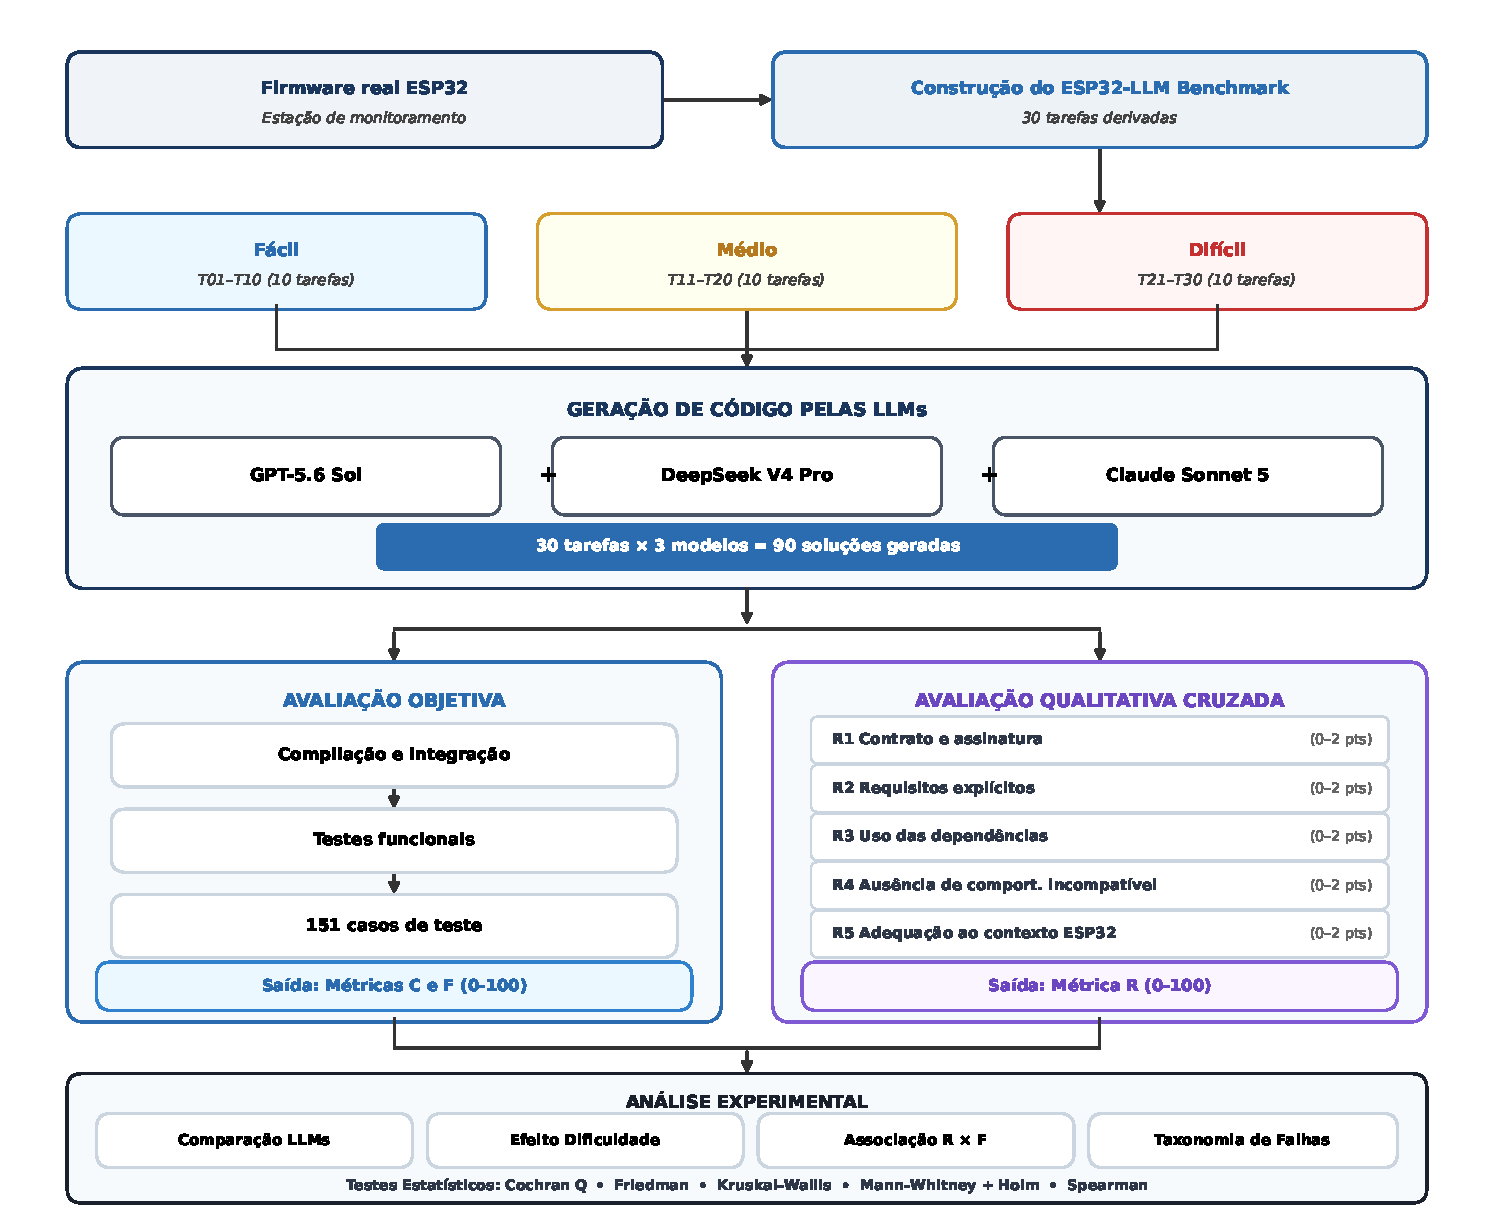
\includegraphics[width=\textwidth]{fluxo_metodologico_esp32_llm_sbc_compacto.pdf}
    \caption{Fluxo metodológico do ESP32-LLM Benchmark.}
    \label{fig:fluxo-metodologico}
\end{figure}

A Figura~\ref{fig:fluxo-metodologico} sintetiza o desenho experimental adotado, desde a derivação das tarefas a partir do firmware de referência até as etapas de geração das soluções, avaliação objetiva, avaliação qualitativa cruzada e análise estatística.

\subsection{ESP32-LLM Benchmark e LLMs}
\label{sec:benchmark}

O ESP32-LLM Benchmark foi construído a partir de um firmware real de uma estação de monitoramento baseada em ESP32, envolvendo aquisição de sensores, cálculos, interrupções, EEPROM, serialização JSON, comunicação HTTP e serviços de configuração. Desse firmware foram derivadas 30 tarefas, cada uma submetida individualmente às LLMs por meio de especificação padronizada, contendo o contrato da tarefa, o contexto necessário e os requisitos esperados. Os casos de teste foram definidos antes da geração das respostas.

As tarefas foram divididas, previamente à geração e avaliação das respostas, em três grupos balanceados. As tarefas fáceis apresentam lógica predominantemente autocontida, interfaces simples e baixa dependência do restante do firmware. As médias acrescentam interação com periféricos, memória, interrupções ou estruturas específicas do sistema, mantendo escopo de integração delimitado. As difíceis combinam maior dependência de estado global, bibliotecas, APIs e contratos de integração com diferentes componentes do firmware. Essa classificação foi estabelecida antes da execução do experimento e não foi modificada com base nos resultados observados. A Tabela~\ref{tab:tarefas} apresenta as unidades experimentais.

\begin{table}[ht]
\centering
\caption{Tarefas que compõem o ESP32-LLM Benchmark.}
\label{tab:tarefas}
\small
\begin{tabular}{lll}
\hline
\textbf{Fácil} & \textbf{Médio} & \textbf{Difícil} \\
\hline
T01 -- passaTesteDegrau       & T11 -- isrPluviometro          & T21 -- setup \\
T02 -- Acumulador             & T12 -- isrAnemometro           & T22 -- loop \\
T03 -- detectarEeprom         & T13 -- identificarChipBmx      & T23 -- inicializarSensores \\
T04 -- lerUV                  & T14 -- lerPressaoAltitude      & T24 -- lerAmbiente \\
T05 -- faixaValida            & T15 -- lerLDR                  & T25 -- coletarAmostra \\
T06 -- calcularPontoOrvalho   & T16 -- calcularIndiceCalor     & T26 -- gravarRegistroPendente \\
T07 -- calcularITGU           & T17 -- escreverEEPROM          & T27 -- montarJSON \\
T08 -- calcularITU            & T18 -- lerEEPROM               & T28 -- enviarParaUmServidor \\
T09 -- classificarIndiceCalor & T19 -- calcularChecksum        & T29 -- tentarDrenarFila \\
T10 -- classificar            & T20 -- lerRegistro             & T30 -- configurarServidorAdmin \\
\hline
\end{tabular}
\end{table}

Foram avaliados GPT-5.6 Sol (LLM01), DeepSeek V4 Pro (LLM02) e Claude Sonnet 5 (LLM03), acessados pelas APIs dos respectivos provedores. Para cada tarefa, o mesmo prompt foi submetido aos três modelos, totalizando 90 soluções. Considerou-se exclusivamente a primeira resposta, sem ciclos de correção, feedback dos testes ou refinamento iterativo, e as respostas originais foram preservadas sem correção manual.

\subsection{Procedimento e Métricas de Avaliação}
\label{sec:procedimento}

A avaliação objetiva utilizou Arduino CLI 1.5.1, core \texttt{esp32:esp32} versão 3.3.8 e FQBN \texttt{esp32:esp32:esp32}. Cada solução foi inicialmente compilada e integrada ao ambiente de teste da tarefa. As soluções compiláveis foram submetidas aos casos funcionais previamente definidos. Dependências externas foram controladas por ambientes de teste e, nas tarefas dependentes de periféricos, utilizou-se uma configuração física padronizada do ESP32, mantendo-se o mesmo circuito e procedimento entre os modelos. Comparações de ponto flutuante utilizaram tolerâncias previamente definidas. No total, o benchmark compreende 151 casos de teste.

Foram mantidas separadas três dimensões, normalizadas entre 0 e 100: compilação e integração ($C$), correção funcional ($F$) e avaliação qualitativa ($R$). Para cada solução, $C=100$ indica compilação bem-sucedida e $C=0$ uma falha que impede os testes. A correção funcional corresponde à proporção de casos aprovados,
\begin{equation}
F = \frac{a}{n} \times 100,
\label{eq:funcional}
\end{equation}
em que $a$ representa os casos aprovados e $n$ o total associado à tarefa. Para fins da métrica, soluções que não compilaram receberam $F=0$, pois não puderam ser submetidas aos testes funcionais. Não foram realizadas modificações manuais no código candidato.

A dimensão $R$ foi obtida por avaliação qualitativa cruzada, separadamente dos resultados de compilação e testes. Cada solução foi avaliada pelas duas LLMs que não a produziram, evitando autoavaliação. Utilizou-se uma rubrica composta por cinco critérios, pontuados de 0 a 2: preservação do contrato e assinatura (R1), atendimento aos requisitos explícitos (R2), uso coerente das dependências fornecidas (R3), ausência de comportamento incompatível (R4) e adequação ao contexto ESP32 e sistemas embarcados (R5). A soma resultou em uma nota entre 0 e 10, posteriormente normalizada para $R$ entre 0 e 100. Foram previstos 180 julgamentos, dos quais 177 foram utilizáveis. Casos com julgamento ausente ou diferença de pelo menos quatro pontos entre os avaliadores, na escala de 0 a 10, foram submetidos à auditoria humana empregando a mesma rubrica, totalizando quatro soluções auditadas. $R$ foi tratado como medida complementar da qualidade percebida e não foi agregado a $C$ e $F$.

\subsection{Análise Estatística}
\label{sec:estatistica}

Como as mesmas 30 tarefas foram submetidas às três LLMs, as comparações entre modelos preservaram o pareamento por tarefa. Adotou-se $\alpha=0{,}05$. O sucesso de compilação foi comparado pelo teste $Q$ de Cochran e $F$ pelo teste de Friedman. Para avaliar o efeito da dificuldade, formada por conjuntos distintos de tarefas, aplicou-se Kruskal--Wallis separadamente a cada LLM, seguido, quando pertinente, por Mann--Whitney com correção de Holm e tamanho de efeito rank-biserial.

A associação entre $R$ e $F$ foi examinada pela correlação de Spearman no conjunto completo e separadamente por dificuldade. A estratificação permite verificar se uma associação global persiste dentro dos níveis. Resultados com $p<0{,}05$ foram considerados significativos; ausência de significância foi interpretada como insuficiência de evidência para rejeitar a hipótese nula, e não como demonstração de equivalência.

\section{Resultados}
\label{sec:resultados}

\subsection{Desempenho Geral}
\label{sec:desempenho-geral}

Considerando as 30 tarefas, o GPT-5.6 Sol apresentou média de $76{,}67$ para compilação e integração ($C$) e $76{,}67$ para correção funcional ($F$). O DeepSeek V4 Pro obteve $C=73{,}33$ e $F=71{,}00$, enquanto o Claude Sonnet 5 apresentou $C=70{,}00$ e $F=70{,}00$. Em números absolutos, 23 das 30 soluções do GPT compilaram, em comparação com 22 do DeepSeek e 21 do Claude.

Essas diferenças devem ser interpretadas descritivamente. Como apresentado na Seção~\ref{sec:resultados-estatisticos}, os testes inferenciais não identificaram diferença estatisticamente significativa entre as três LLMs para compilação ou correção funcional. Portanto, os resultados não fornecem evidência suficiente para estabelecer superioridade global de um dos modelos avaliados.

A Figura~\ref{fig:rcf-modelo-nivel} apresenta conjuntamente as métricas $R$, $C$ e $F$ segundo modelo e nível de dificuldade, permitindo observar que a maior variação de desempenho ocorre nas tarefas difíceis.

\begin{figure}[ht]
\centering
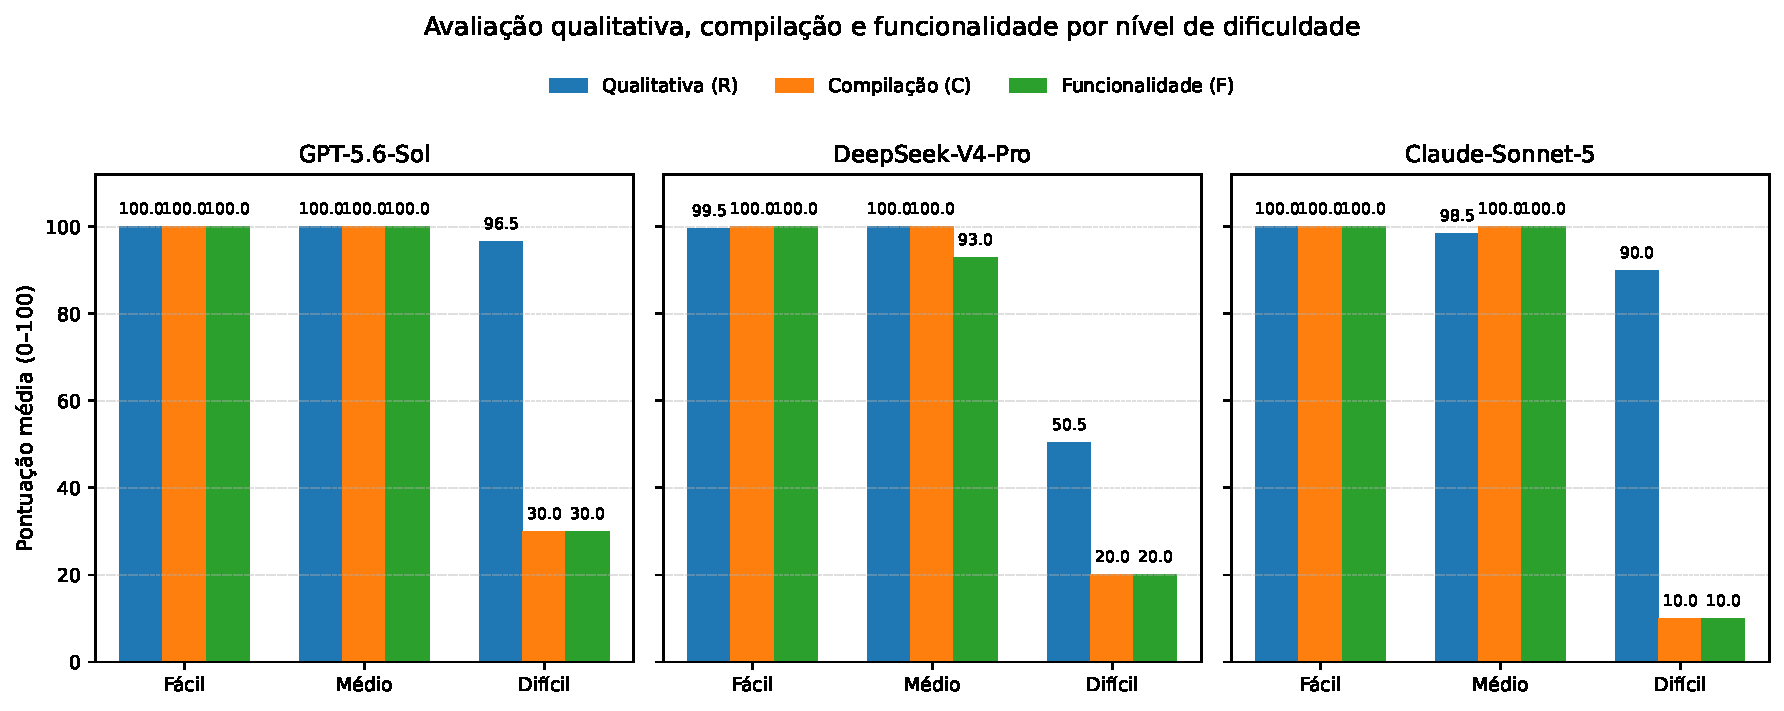
\includegraphics[width=0.98\columnwidth]{../../../16-figuras-resultados/figura_01_R_C_F_por_modelo_nivel.pdf}
\caption{Médias de avaliação qualitativa ($R$), compilação ($C$) e correção funcional ($F$) por modelo e nível de dificuldade.}
\label{fig:rcf-modelo-nivel}
\end{figure}

\subsection{Efeito do Nível de Dificuldade}
\label{sec:efeito-dificuldade}

Nas tarefas fáceis, os três modelos apresentaram $C=100$ e $F=100$, indicando que todas as soluções compilaram e foram aprovadas nos respectivos casos de teste. Nas tarefas médias, GPT-5.6 Sol e Claude Sonnet 5 também mantiveram $C=100$ e $F=100$. O DeepSeek V4 Pro apresentou $C=100$ e $F=93$, devido a falhas funcionais parciais nas tarefas T13 e T14, que obtiveram, respectivamente, $F=80$ e $F=50$.

A maior redução ocorreu no nível difícil. O GPT-5.6 Sol apresentou $C=30$ e $F=30$, o DeepSeek V4 Pro $C=20$ e $F=20$, e o Claude Sonnet 5 $C=10$ e $F=10$. Das 30 combinações entre modelos e tarefas desse nível, apenas seis compilaram e foram aprovadas integralmente nos testes funcionais, enquanto 24 não atingiram a etapa de testes funcionais em razão de falha registrada na etapa de compilação ou integração.

Não foram observadas, nesse subconjunto, soluções que compilassem e apresentassem aprovação apenas parcial nos testes funcionais. Assim, a redução de $F$ nas tarefas difíceis decorreu predominantemente de falhas que impediram a execução dos testes, e não de uma degradação gradual da correção funcional entre soluções compiláveis. A Figura~\ref{fig:funcional-dificuldade} evidencia essa mudança de desempenho entre os níveis.

\begin{figure}[ht]
\centering
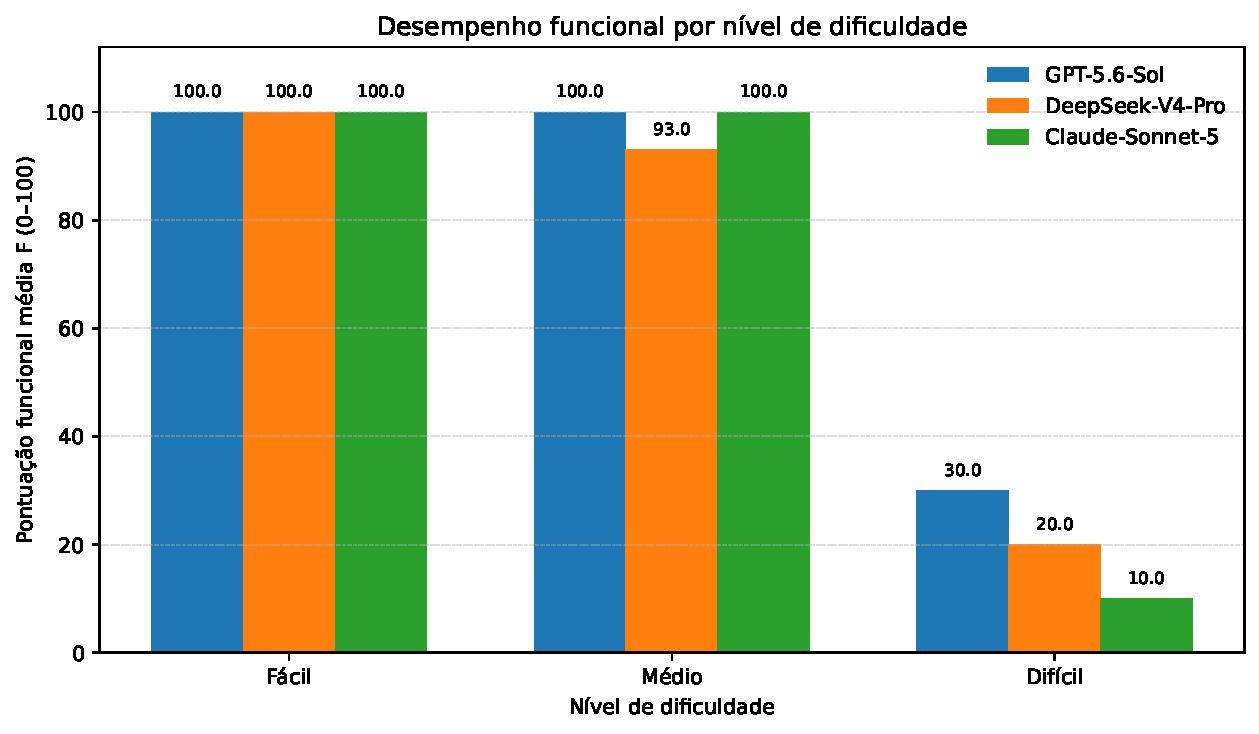
\includegraphics[width=0.90\columnwidth]{../../../16-figuras-resultados/figura_02_funcionalidade_por_dificuldade.pdf}
\caption{Correção funcional ($F$) das LLMs nos três níveis de dificuldade.}
\label{fig:funcional-dificuldade}
\end{figure}

A análise por tarefa mostra ainda que o sucesso no nível difícil ficou concentrado em poucas unidades do benchmark. A T28 foi a única tarefa difícil aprovada pelos três modelos; a T22 foi aprovada pelo GPT-5.6 Sol e pelo DeepSeek V4 Pro; e a T21 foi aprovada apenas pelo GPT-5.6 Sol. As tarefas T23--T27, T29 e T30 não apresentaram sucesso objetivo para nenhum dos três modelos.

\subsection{Análise Estatística}
\label{sec:resultados-estatisticos}

A comparação global entre as LLMs não revelou diferença estatisticamente significativa. Para compilação, o teste $Q$ de Cochran resultou em $Q=3{,}00$ e $p=0{,}223$; para correção funcional, o teste de Friedman produziu $\chi^2=3{,}50$ e $p=0{,}174$. Portanto, as diferenças descritivas observadas entre os modelos não constituem evidência de superioridade global de uma LLM neste experimento.

Em contraste, o efeito da dificuldade sobre $F$ foi significativo para os três modelos: GPT-5.6 Sol ($H=17{,}65$, $p<0{,}001$), DeepSeek V4 Pro ($H=17{,}64$, $p<0{,}001$) e Claude Sonnet 5 ($H=24{,}86$, $p<0{,}001$).

Nas comparações par a par com correção de Holm, as diferenças envolvendo o nível difícil permaneceram significativas. Para GPT, fácil--difícil e médio--difícil apresentaram $p_{\mathrm{Holm}}=0{,}0032$; para DeepSeek, $p_{\mathrm{Holm}}=0{,}0013$ e $0{,}0033$, respectivamente; e, para Claude, ambas apresentaram $p_{\mathrm{Holm}}<0{,}001$. A comparação fácil--médio do DeepSeek não foi significativa ($p_{\mathrm{Holm}}=0{,}168$).

Os tamanhos de efeito rank-biserial nas comparações com o nível difícil foram elevados: $0{,}70$ para GPT nas comparações fácil--difícil e médio--difícil; $0{,}80$ e $0{,}76$ para DeepSeek; e $0{,}90$ para Claude em ambas as comparações. Os resultados inferenciais, portanto, corroboram a análise descritiva de que a principal variação de desempenho está associada às tarefas classificadas como difíceis.

\subsection{Falhas nas Tarefas Difíceis}
\label{sec:falhas}

A análise das tarefas difíceis mostra que o problema predominante não esteve associado apenas à implementação da lógica local, mas à integração das soluções ao contexto do firmware. Das 30 combinações modelo--tarefa desse nível, seis resultaram em sucesso completo e 24 apresentaram falha de compilação ou integração.

Foi possível classificar de forma conclusiva 21 dessas 24 falhas. Entre elas, 16 ($76{,}2\%$) foram classificadas como incompatibilidade contextual (E3), caracterizada por divergências em nomes, campos, estado compartilhado, constantes, tipos ou contratos esperados pelo firmware. Três falhas ($14{,}3\%$) decorreram de implementação ausente ou incompleta (E2), e duas ($9{,}5\%$) foram associadas ao uso incompatível de APIs ou bibliotecas (E1). As três falhas restantes, referentes à tarefa T24, foram mantidas como indeterminadas e não foram incluídas no cálculo dessas proporções.

\begin{figure}[ht]
\centering
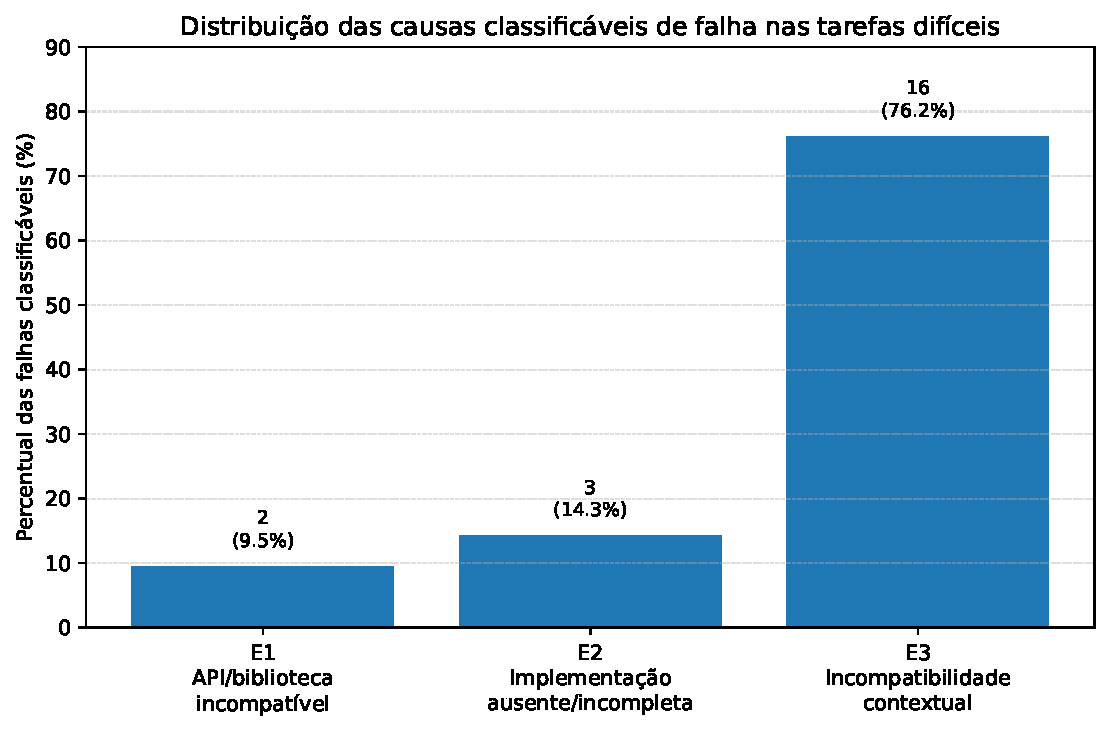
\includegraphics[width=0.88\columnwidth]{../../../16-figuras-resultados/figura_04_taxonomia_falhas_dificeis.pdf}
\caption{Distribuição das categorias de falha entre as ocorrências classificáveis nas tarefas difíceis.}
\label{fig:taxonomia-falhas}
\end{figure}

O predomínio de E3 sugere que, para as tarefas difíceis deste benchmark, preservar corretamente os contratos e dependências do firmware constituiu uma dificuldade mais frequente do que produzir apenas a lógica local solicitada.

\subsection{Avaliação Qualitativa e Desempenho Objetivo}
\label{sec:qualitativa-objetiva}

A comparação entre a avaliação qualitativa ($R$) e a correção funcional ($F$) revelou uma associação global positiva, com correlação de Spearman $\rho=0{,}658$ ($p<0{,}001$, $N=90$). Entretanto, esse resultado deve ser interpretado considerando a forte separação de desempenho entre os níveis de dificuldade.

Quando a análise foi realizada separadamente por nível, não foi possível calcular uma correlação informativa para as tarefas fáceis, pois $F$ permaneceu constante em 100. Nas tarefas médias, a associação foi praticamente nula ($\rho=-0{,}050$, $p=0{,}795$), enquanto nas difíceis foi positiva, porém fraca e não significativa ($\rho=0{,}292$, $p=0{,}117$).

Esses resultados indicam que a correlação global entre $R$ e $F$ é influenciada, ao menos em parte, pelas diferenças entre os níveis de dificuldade. Portanto, não há evidência suficiente para concluir que uma avaliação qualitativa elevada seja, isoladamente, um indicador confiável de compilação e correção funcional.

Essa divergência torna-se particularmente evidente nas tarefas difíceis. O GPT-5.6 Sol apresentou média qualitativa $R=96{,}5$, embora tenha obtido apenas $C=30$ e $F=30$. O Claude Sonnet 5 apresentou $R=90{,}0$, com $C=10$ e $F=10$. O DeepSeek V4 Pro apresentou menor avaliação qualitativa nesse nível ($R=50{,}5$), com $C=20$ e $F=20$. Foram identificadas ainda 18 soluções com $R\geq80$ e $F<100$, utilizadas apenas como análise descritiva exploratória.

Em conjunto, esses resultados mostram que uma solução pode apresentar estrutura aparentemente adequada, preservar parte dos requisitos e receber avaliação qualitativa elevada, mas ainda assim falhar ao ser compilada ou integrada ao firmware alvo. Esse resultado reforça a necessidade de combinar inspeção qualitativa com evidências executáveis na avaliação de código gerado por LLMs para sistemas embarcados.

\section{Discussão}
\label{sec:discussao}

Os resultados permitem responder às quatro questões de pesquisa propostas. Em relação à \textbf{RQ1}, os três modelos apresentaram desempenho global relativamente próximo. Embora o GPT-5.6 Sol tenha obtido os maiores valores descritivos de compilação e correção funcional, seguido por DeepSeek V4 Pro e Claude Sonnet 5, os testes de Cochran e Friedman não identificaram diferenças estatisticamente significativas entre as LLMs. Assim, os resultados deste experimento não sustentam a afirmação de superioridade global de um modelo. Da mesma forma, a ausência de significância estatística não deve ser interpretada como demonstração de equivalência entre os modelos.

Quanto à \textbf{RQ2}, a dificuldade das tarefas apresentou efeito expressivo sobre o desempenho. Todos os modelos resolveram integralmente as tarefas fáceis e mantiveram desempenho elevado no nível médio. A principal ruptura ocorreu no nível difícil, no qual somente 6 das 30 combinações modelo--tarefa compilaram e passaram integralmente nos testes. O efeito da dificuldade foi estatisticamente significativo para os três modelos e acompanhado por tamanhos de efeito elevados nas comparações envolvendo o nível difícil. Esse comportamento é compatível com a observação de que tarefas de programação embarcada se tornam mais desafiadoras quando aumentam as dependências de hardware, APIs e contexto de integração \cite{babiuch2026benchmarking}.

Um aspecto relevante é que a queda observada nas tarefas difíceis não se manifestou principalmente como redução gradual na quantidade de casos funcionais aprovados. Das 30 observações desse nível, 24 falharam antes da execução dos testes funcionais, na etapa de compilação ou integração. Portanto, no contexto deste benchmark, o aumento da dificuldade esteve associado principalmente à capacidade de produzir uma solução compatível com o ambiente completo do firmware, e não apenas à implementação da lógica local solicitada.

Para a \textbf{RQ3}, a correlação global entre avaliação qualitativa e desempenho funcional foi positiva. Entretanto, a associação não se manteve quando os níveis médio e difícil foram examinados separadamente. Particularmente nas tarefas difíceis, foram observadas pontuações qualitativas elevadas em soluções que não compilaram ou não puderam ser corretamente integradas. Esse resultado evidencia que inspeções qualitativas e testes executáveis capturam propriedades distintas do código gerado. Consequentemente, uma avaliação qualitativa favorável não deve substituir a compilação e a validação funcional no ambiente alvo.

Em resposta à \textbf{RQ4}, a incompatibilidade contextual (E3) foi a categoria predominante entre as falhas cuja causa pôde ser determinada, representando 16 das 21 ocorrências classificáveis. Essas falhas envolveram contratos, nomes, campos, tipos, constantes, estado compartilhado ou outros elementos necessários à integração com o firmware. Implementações ausentes ou incompletas e incompatibilidades de APIs ou bibliotecas ocorreram com menor frequência. O resultado indica que, nas tarefas mais dependentes do sistema, fornecer uma implementação local aparentemente plausível não é suficiente: a solução precisa preservar os contratos do contexto no qual será incorporada.

Em conjunto, os resultados sugerem que benchmarks de geração de código para sistemas embarcados podem se beneficiar de tarefas que ultrapassem funções autocontidas e incluam dependências reais de um firmware. Nesse cenário, compilação, integração e testes funcionais fornecem evidências complementares à inspeção qualitativa e permitem identificar falhas que poderiam permanecer ocultas em uma avaliação baseada somente na aparência ou estrutura do código.

\section{Ameaças à Validade}
\label{sec:ameacas}

Como ameaça à validade de construção, a classificação das tarefas em fácil, médio e difícil representa uma operacionalização da dificuldade baseada nas características do firmware, como dependência de periféricos, estado compartilhado, bibliotecas e contratos de integração. Embora essa classificação tenha sido estabelecida antes da execução do experimento, outros critérios de dificuldade poderiam produzir agrupamentos diferentes. Além disso, $R$, $C$ e $F$ representam dimensões distintas e não devem ser interpretadas como uma medida única de qualidade.

Quanto à validade interna, buscou-se manter constantes os prompts, os casos de teste, a regra de utilização apenas da primeira resposta e o ambiente de compilação. Ainda assim, resultados de LLMs podem depender da versão disponibilizada pelo provedor e de aspectos não controláveis de sua infraestrutura. O ambiente experimental foi congelado com Arduino CLI 1.5.1, core ESP32 3.3.8 e FQBN \texttt{esp32:esp32:esp32}, reduzindo variações associadas à cadeia de compilação.

Durante a validação da T27 foi identificada a ausência da dependência ArduinoJson no ambiente de teste. A versão 6.21.6 foi então instalada e o teste foi repetido para os três modelos sem modificação das respostas geradas. Após a correção da infraestrutura, as três soluções continuaram apresentando falha, permitindo separar o problema experimental inicial das incompatibilidades efetivamente presentes nos candidatos.

Para a T24, uma discrepância foi identificada entre uma execução posterior do script de teste e o conjunto consolidado utilizado na análise. Os resultados oficiais preservados registram falha de compilação para os três modelos, mas a evidência disponível não permitiu reconstruir com segurança a causa específica dessas falhas. Por essa razão, as três ocorrências foram mantidas como indeterminadas na taxonomia e nenhuma causa específica foi atribuída retrospectivamente. Essa decisão reduz o risco de introduzir explicações não sustentadas pelos artefatos preservados.

A avaliação qualitativa também está sujeita à subjetividade dos avaliadores. Para reduzir essa ameaça, cada resposta foi avaliada pelas duas LLMs que não a produziram, utilizando a mesma rubrica. Casos com ausência de julgamento ou discordância elevada foram submetidos à auditoria humana. Ainda assim, a utilização de LLMs como avaliadores pode introduzir vieses compartilhados entre geração e julgamento.

Por fim, a validade externa é limitada pelo fato de as 30 tarefas terem sido derivadas de um único firmware ESP32. Embora elas cubram diferentes funcionalidades e graus de dependência contextual, os resultados não devem ser generalizados automaticamente para outros microcontroladores, frameworks, linguagens ou domínios. Estudos futuros devem replicar o protocolo em diferentes firmwares e plataformas embarcadas.

\section{Conclusão}
\label{sec:conclusao}

Este trabalho apresentou o ESP32-LLM Benchmark, um estudo experimental para avaliar a confiabilidade de código gerado por LLMs em tarefas derivadas de um firmware ESP32 real. Foram avaliadas 90 soluções produzidas por GPT-5.6 Sol, DeepSeek V4 Pro e Claude Sonnet 5 em 30 tarefas distribuídas igualmente entre os níveis fácil, médio e difícil. A avaliação combinou compilação e integração, 151 casos de teste funcionais, avaliação qualitativa cruzada e análise estatística.

Os três modelos apresentaram desempenho elevado nas tarefas fáceis e médias, mas uma redução acentuada nas tarefas difíceis. Não foram identificadas diferenças estatisticamente significativas entre as LLMs em compilação ou correção funcional global. Em contraste, a dificuldade apresentou efeito significativo para os três modelos. Nas tarefas difíceis, 24 das 30 combinações modelo--tarefa falharam na compilação ou integração, e a incompatibilidade contextual foi a causa predominante entre as ocorrências de falha que puderam ser classificadas.

A comparação entre avaliação qualitativa e comportamento executável mostrou ainda que soluções bem avaliadas qualitativamente podem apresentar falhas objetivas. Assim, no contexto analisado, a confiabilidade do código gerado não pode ser inferida apenas por inspeção qualitativa, sendo necessário confrontar as soluções com o ambiente de compilação, os contratos de integração e os testes funcionais do sistema alvo.

Como trabalhos futuros, pretende-se ampliar o benchmark para diferentes firmwares e plataformas embarcadas, incluir novas LLMs e investigar estratégias de prompting que forneçam maior contexto de integração. Também é relevante avaliar se mecanismos de geração iterativa, recuperação de contexto e feedback de compilação conseguem reduzir as incompatibilidades observadas nas tarefas de maior complexidade.

\bibliographystyle{sbc}
\bibliography{sbc-template}

\end{document}


